\documentclass[1p]{elsarticle_modified}
%\bibliographystyle{elsarticle-num}

%\usepackage[colorlinks]{hyperref}
%\usepackage{abbrmath_seonhwa} %\Abb, \Ascr, \Acal ,\Abf, \Afrak
\usepackage{amsfonts}
\usepackage{amssymb}
\usepackage{amsmath}
\usepackage{amsthm}
\usepackage{scalefnt}
\usepackage{amsbsy}
\usepackage{kotex}
\usepackage{caption}
\usepackage{subfig}
\usepackage{color}
\usepackage{graphicx}
\usepackage{xcolor} %% white, black, red, green, blue, cyan, magenta, yellow
\usepackage{float}
\usepackage{setspace}
\usepackage{hyperref}

\usepackage{tikz}
\usetikzlibrary{arrows}

\usepackage{multirow}
\usepackage{array} % fixed length table
\usepackage{hhline}

%%%%%%%%%%%%%%%%%%%%%
\makeatletter
\renewcommand*\env@matrix[1][\arraystretch]{%
	\edef\arraystretch{#1}%
	\hskip -\arraycolsep
	\let\@ifnextchar\new@ifnextchar
	\array{*\c@MaxMatrixCols c}}
\makeatother %https://tex.stackexchange.com/questions/14071/how-can-i-increase-the-line-spacing-in-a-matrix
%%%%%%%%%%%%%%%

\usepackage[normalem]{ulem}

\newcommand{\msout}[1]{\ifmmode\text{\sout{\ensuremath{#1}}}\else\sout{#1}\fi}
%SOURCE: \msout is \stkout macro in https://tex.stackexchange.com/questions/20609/strikeout-in-math-mode

\newcommand{\cancel}[1]{
	\ifmmode
	{\color{red}\msout{#1}}
	\else
	{\color{red}\sout{#1}}
	\fi
}

\newcommand{\add}[1]{
	{\color{blue}\uwave{#1}}
}

\newcommand{\replace}[2]{
	\ifmmode
	{\color{red}\msout{#1}}{\color{blue}\uwave{#2}}
	\else
	{\color{red}\sout{#1}}{\color{blue}\uwave{#2}}
	\fi
}

\newcommand{\Sol}{\mathcal{S}} %segment
\newcommand{\D}{D} %diagram
\newcommand{\A}{\mathcal{A}} %arc


%%%%%%%%%%%%%%%%%%%%%%%%%%%%%5 test

\def\sl{\operatorname{\textup{SL}}(2,\Cbb)}
\def\psl{\operatorname{\textup{PSL}}(2,\Cbb)}
\def\quan{\mkern 1mu \triangleright \mkern 1mu}

\theoremstyle{definition}
\newtheorem{thm}{Theorem}[section]
\newtheorem{prop}[thm]{Proposition}
\newtheorem{lem}[thm]{Lemma}
\newtheorem{ques}[thm]{Question}
\newtheorem{cor}[thm]{Corollary}
\newtheorem{defn}[thm]{Definition}
\newtheorem{exam}[thm]{Example}
\newtheorem{rmk}[thm]{Remark}
\newtheorem{alg}[thm]{Algorithm}

\newcommand{\I}{\sqrt{-1}}
\begin{document}

%\begin{frontmatter}
%
%\title{Boundary parabolic representations of knots up to 8 crossings}
%
%%% Group authors per affiliation:
%\author{Yunhi Cho} 
%\address{Department of Mathematics, University of Seoul, Seoul, Korea}
%\ead{yhcho@uos.ac.kr}
%
%
%\author{Seonhwa Kim} %\fnref{s_kim}}
%\address{Center for Geometry and Physics, Institute for Basic Science, Pohang, 37673, Korea}
%\ead{ryeona17@ibs.re.kr}
%
%\author{Hyuk Kim}
%\address{Department of Mathematical Sciences, Seoul National University, Seoul 08826, Korea}
%\ead{hyukkim@snu.ac.kr}
%
%\author{Seokbeom Yoon}
%\address{Department of Mathematical Sciences, Seoul National University, Seoul, 08826,  Korea}
%\ead{sbyoon15@snu.ac.kr}
%
%\begin{abstract}
%We find all boundary parabolic representation of knots up to 8 crossings.
%
%\end{abstract}
%\begin{keyword}
%    \MSC[2010] 57M25 
%\end{keyword}
%
%\end{frontmatter}

%\linenumbers
%\tableofcontents
%
\newcommand\colored[1]{\textcolor{white}{\rule[-0.35ex]{0.8em}{1.4ex}}\kern-0.8em\color{red} #1}%
%\newcommand\colored[1]{\textcolor{white}{ #1}\kern-2.17ex	\textcolor{white}{ #1}\kern-1.81ex	\textcolor{white}{ #1}\kern-2.15ex\color{red}#1	}

{\Large $\underline{12a_{0541}~(K12a_{0541})}$}

\setlength{\tabcolsep}{10pt}
\renewcommand{\arraystretch}{1.6}
\vspace{1cm}\begin{tabular}{m{100pt}>{\centering\arraybackslash}m{274pt}}
\multirow{5}{120pt}{
	\centering
	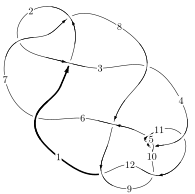
\includegraphics[width=112pt]{../../../GIT/diagram.site/Diagrams/png/1342_12a_0541.png}\\
\ \ \ A knot diagram\footnotemark}&
\allowdisplaybreaks
\textbf{Linearized knot diagam} \\
\cline{2-2}
 &
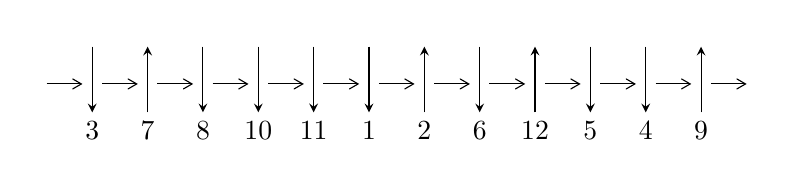
\begin{tikzpicture}[x=20pt, y=17pt]
	% nodes
	\node (C0) at (0, 0) {};
	\node (C1) at (1, 0) {};
	\node (C1U) at (1, +1) {};
	\node (C1D) at (1, -1) {3};

	\node (C2) at (2, 0) {};
	\node (C2U) at (2, +1) {};
	\node (C2D) at (2, -1) {7};

	\node (C3) at (3, 0) {};
	\node (C3U) at (3, +1) {};
	\node (C3D) at (3, -1) {8};

	\node (C4) at (4, 0) {};
	\node (C4U) at (4, +1) {};
	\node (C4D) at (4, -1) {10};

	\node (C5) at (5, 0) {};
	\node (C5U) at (5, +1) {};
	\node (C5D) at (5, -1) {11};

	\node (C6) at (6, 0) {};
	\node (C6U) at (6, +1) {};
	\node (C6D) at (6, -1) {1};

	\node (C7) at (7, 0) {};
	\node (C7U) at (7, +1) {};
	\node (C7D) at (7, -1) {2};

	\node (C8) at (8, 0) {};
	\node (C8U) at (8, +1) {};
	\node (C8D) at (8, -1) {6};

	\node (C9) at (9, 0) {};
	\node (C9U) at (9, +1) {};
	\node (C9D) at (9, -1) {12};

	\node (C10) at (10, 0) {};
	\node (C10U) at (10, +1) {};
	\node (C10D) at (10, -1) {5};

	\node (C11) at (11, 0) {};
	\node (C11U) at (11, +1) {};
	\node (C11D) at (11, -1) {4};

	\node (C12) at (12, 0) {};
	\node (C12U) at (12, +1) {};
	\node (C12D) at (12, -1) {9};
	\node (C13) at (13, 0) {};

	% arrows
	\draw[->,>={angle 60}]
	(C0) edge (C1) (C1) edge (C2) (C2) edge (C3) (C3) edge (C4) (C4) edge (C5) (C5) edge (C6) (C6) edge (C7) (C7) edge (C8) (C8) edge (C9) (C9) edge (C10) (C10) edge (C11) (C11) edge (C12) (C12) edge (C13) ;	\draw[->,>=stealth]
	(C1U) edge (C1D) (C2D) edge (C2U) (C3U) edge (C3D) (C4U) edge (C4D) (C5U) edge (C5D) (C6U) edge (C6D) (C7D) edge (C7U) (C8U) edge (C8D) (C9D) edge (C9U) (C10U) edge (C10D) (C11U) edge (C11D) (C12D) edge (C12U) ;
	\end{tikzpicture} \\
\hhline{~~} \\& 
\textbf{Solving Sequence} \\ \cline{2-2} 
 &
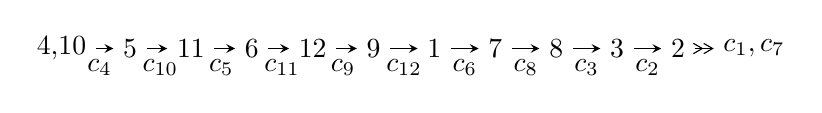
\begin{tikzpicture}[x=22pt, y=7pt]
	% node
	\node (A0) at (-1/8, 0) {4,10};
	\node (A1) at (1, 0) {5};
	\node (A2) at (2, 0) {11};
	\node (A3) at (3, 0) {6};
	\node (A4) at (4, 0) {12};
	\node (A5) at (5, 0) {9};
	\node (A6) at (6, 0) {1};
	\node (A7) at (7, 0) {7};
	\node (A8) at (8, 0) {8};
	\node (A9) at (9, 0) {3};
	\node (A10) at (10, 0) {2};
	\node (C1) at (1/2, -1) {$c_{4}$};
	\node (C2) at (3/2, -1) {$c_{10}$};
	\node (C3) at (5/2, -1) {$c_{5}$};
	\node (C4) at (7/2, -1) {$c_{11}$};
	\node (C5) at (9/2, -1) {$c_{9}$};
	\node (C6) at (11/2, -1) {$c_{12}$};
	\node (C7) at (13/2, -1) {$c_{6}$};
	\node (C8) at (15/2, -1) {$c_{8}$};
	\node (C9) at (17/2, -1) {$c_{3}$};
	\node (C10) at (19/2, -1) {$c_{2}$};
	\node (A11) at (45/4, 0) {$c_{1},c_{7}$};

	% edge
	\draw[->,>=stealth]	
	(A0) edge (A1) (A1) edge (A2) (A2) edge (A3) (A3) edge (A4) (A4) edge (A5) (A5) edge (A6) (A6) edge (A7) (A7) edge (A8) (A8) edge (A9) (A9) edge (A10) ;
	\draw[->>,>={angle 60}]	
	(A10) edge (A11);
\end{tikzpicture} \\ 

\end{tabular} \\

\footnotetext{
The image of knot diagram is generated by the software ``\textbf{Draw programme}" developed by Andrew Bartholomew(\url{http://www.layer8.co.uk/maths/draw/index.htm\#Running-draw}), where we modified some parts for our purpose(\url{https://github.com/CATsTAILs/LinksPainter}).
}\phantom \\ \newline 
\centering \textbf{Ideals for irreducible components\footnotemark of $X_{\text{par}}$} 
 
\begin{align*}
I^u_{1}&=\langle 
u^{76}- u^{75}+\cdots-2 u-1\rangle \\
\\
\end{align*}
\raggedright * 1 irreducible components of $\dim_{\mathbb{C}}=0$, with total 76 representations.\\
\footnotetext{All coefficients of polynomials are rational numbers. But the coefficients are sometimes approximated in decimal forms when there is not enough margin.}
\newpage
\renewcommand{\arraystretch}{1}
\centering \section*{I. $I^u_{1}= \langle u^{76}- u^{75}+\cdots-2 u-1 \rangle$}
\flushleft \textbf{(i) Arc colorings}\\
\begin{tabular}{m{7pt} m{180pt} m{7pt} m{180pt} }
\flushright $a_{4}=$&$\begin{pmatrix}1\\0\end{pmatrix}$ \\
\flushright $a_{10}=$&$\begin{pmatrix}0\\u\end{pmatrix}$ \\
\flushright $a_{5}=$&$\begin{pmatrix}1\\u^2\end{pmatrix}$ \\
\flushright $a_{11}=$&$\begin{pmatrix}- u\\- u^3+u\end{pmatrix}$ \\
\flushright $a_{6}=$&$\begin{pmatrix}- u^2+1\\- u^4+2 u^2\end{pmatrix}$ \\
\flushright $a_{12}=$&$\begin{pmatrix}u^3-2 u\\- u^3+u\end{pmatrix}$ \\
\flushright $a_{9}=$&$\begin{pmatrix}- u^7+4 u^5-4 u^3\\u^7-3 u^5+2 u^3+u\end{pmatrix}$ \\
\flushright $a_{1}=$&$\begin{pmatrix}u^{11}-6 u^9+12 u^7-8 u^5+u^3-2 u\\- u^{11}+5 u^9-8 u^7+3 u^5+u^3+u\end{pmatrix}$ \\
\flushright $a_{7}=$&$\begin{pmatrix}u^{26}-13 u^{24}+\cdots-3 u^2+1\\- u^{26}+12 u^{24}+\cdots+4 u^4+3 u^2\end{pmatrix}$ \\
\flushright $a_{8}=$&$\begin{pmatrix}u^{13}-6 u^{11}+13 u^9-12 u^7+6 u^5-4 u^3+u\\u^{15}-7 u^{13}+18 u^{11}-19 u^9+6 u^7-2 u^5+4 u^3+u\end{pmatrix}$ \\
\flushright $a_{3}=$&$\begin{pmatrix}- u^{28}+13 u^{26}+\cdots- u^2+1\\- u^{30}+14 u^{28}+\cdots-8 u^4- u^2\end{pmatrix}$ \\
\flushright $a_{2}=$&$\begin{pmatrix}u^{69}-32 u^{67}+\cdots+4 u^3-3 u\\u^{71}-33 u^{69}+\cdots+2 u^3+u\end{pmatrix}$\\&\end{tabular}
\flushleft \textbf{(ii) Obstruction class $= -1$}\\~\\
\flushleft \textbf{(iii) Cusp Shapes $= -4 u^{74}+140 u^{72}+\cdots-20 u-10$}\\~\\
\newpage\renewcommand{\arraystretch}{1}
\flushleft \textbf{(iv) u-Polynomials at the component}\newline \\
\begin{tabular}{m{50pt}|m{274pt}}
Crossings & \hspace{64pt}u-Polynomials at each crossing \\
\hline $$\begin{aligned}c_{1}\end{aligned}$$&$\begin{aligned}
&u^{76}+41 u^{75}+\cdots+2 u+1
\end{aligned}$\\
\hline $$\begin{aligned}c_{2},c_{7}\end{aligned}$$&$\begin{aligned}
&u^{76}+u^{75}+\cdots-2 u-1
\end{aligned}$\\
\hline $$\begin{aligned}c_{3},c_{6}\end{aligned}$$&$\begin{aligned}
&u^{76}- u^{75}+\cdots+u-2
\end{aligned}$\\
\hline $$\begin{aligned}c_{4},c_{5},c_{10}\end{aligned}$$&$\begin{aligned}
&u^{76}- u^{75}+\cdots-2 u-1
\end{aligned}$\\
\hline $$\begin{aligned}c_{8}\end{aligned}$$&$\begin{aligned}
&u^{76}-11 u^{75}+\cdots-5222 u+701
\end{aligned}$\\
\hline $$\begin{aligned}c_{9},c_{12}\end{aligned}$$&$\begin{aligned}
&u^{76}+11 u^{75}+\cdots+28 u+1
\end{aligned}$\\
\hline $$\begin{aligned}c_{11}\end{aligned}$$&$\begin{aligned}
&u^{76}+3 u^{75}+\cdots+1213 u+264
\end{aligned}$\\
\hline
\end{tabular}\\~\\
\newpage\renewcommand{\arraystretch}{1}
\flushleft \textbf{(v) Riley Polynomials at the component}\newline \\
\begin{tabular}{m{50pt}|m{274pt}}
Crossings & \hspace{64pt}Riley Polynomials at each crossing \\
\hline $$\begin{aligned}c_{1}\end{aligned}$$&$\begin{aligned}
&y^{76}-11 y^{75}+\cdots-10 y+1
\end{aligned}$\\
\hline $$\begin{aligned}c_{2},c_{7}\end{aligned}$$&$\begin{aligned}
&y^{76}+41 y^{75}+\cdots+2 y+1
\end{aligned}$\\
\hline $$\begin{aligned}c_{3},c_{6}\end{aligned}$$&$\begin{aligned}
&y^{76}-63 y^{75}+\cdots+659 y+4
\end{aligned}$\\
\hline $$\begin{aligned}c_{4},c_{5},c_{10}\end{aligned}$$&$\begin{aligned}
&y^{76}-71 y^{75}+\cdots+2 y+1
\end{aligned}$\\
\hline $$\begin{aligned}c_{8}\end{aligned}$$&$\begin{aligned}
&y^{76}-23 y^{75}+\cdots+1083362 y+491401
\end{aligned}$\\
\hline $$\begin{aligned}c_{9},c_{12}\end{aligned}$$&$\begin{aligned}
&y^{76}+65 y^{75}+\cdots+174 y+1
\end{aligned}$\\
\hline $$\begin{aligned}c_{11}\end{aligned}$$&$\begin{aligned}
&y^{76}-27 y^{75}+\cdots-2910169 y+69696
\end{aligned}$\\
\hline
\end{tabular}\\~\\
\newpage\flushleft \textbf{(vi) Complex Volumes and Cusp Shapes}
$$\begin{array}{c|c|c}  
\text{Solutions to }I^u_{1}& \I (\text{vol} + \sqrt{-1}CS) & \text{Cusp shape}\\
 \hline 
\begin{aligned}
u &= \phantom{-}1.129570 + 0.058336 I\end{aligned}
 & -4.97762 + 3.97568 I & \phantom{-0.000000 } 0 \\ \hline\begin{aligned}
u &= \phantom{-}1.129570 - 0.058336 I\end{aligned}
 & -4.97762 - 3.97568 I & \phantom{-0.000000 } 0 \\ \hline\begin{aligned}
u &= -0.407771 + 0.685752 I\end{aligned}
 & -8.10020 + 11.53670 I & -9.08879 - 9.10866 I \\ \hline\begin{aligned}
u &= -0.407771 - 0.685752 I\end{aligned}
 & -8.10020 - 11.53670 I & -9.08879 + 9.10866 I \\ \hline\begin{aligned}
u &= -0.419176 + 0.676793 I\end{aligned}
 & -8.93857 + 2.57784 I & -10.57384 - 2.81236 I \\ \hline\begin{aligned}
u &= -0.419176 - 0.676793 I\end{aligned}
 & -8.93857 - 2.57784 I & -10.57384 + 2.81236 I \\ \hline\begin{aligned}
u &= \phantom{-}0.408279 + 0.677761 I\end{aligned}
 & -4.89911 - 6.69327 I & -6.12847 + 6.07369 I \\ \hline\begin{aligned}
u &= \phantom{-}0.408279 - 0.677761 I\end{aligned}
 & -4.89911 + 6.69327 I & -6.12847 - 6.07369 I \\ \hline\begin{aligned}
u &= -1.207110 + 0.068967 I\end{aligned}
 & -2.20534 + 0.18555 I & \phantom{-0.000000 } 0 \\ \hline\begin{aligned}
u &= -1.207110 - 0.068967 I\end{aligned}
 & -2.20534 - 0.18555 I & \phantom{-0.000000 } 0 \\ \hline\begin{aligned}
u &= -0.510556 + 0.594333 I\end{aligned}
 & -9.30162 + 1.64723 I & -11.54189 - 3.42806 I \\ \hline\begin{aligned}
u &= -0.510556 - 0.594333 I\end{aligned}
 & -9.30162 - 1.64723 I & -11.54189 + 3.42806 I \\ \hline\begin{aligned}
u &= -0.525486 + 0.580123 I\end{aligned}
 & -8.56487 - 7.31358 I & -10.37548 + 3.04110 I \\ \hline\begin{aligned}
u &= -0.525486 - 0.580123 I\end{aligned}
 & -8.56487 + 7.31358 I & -10.37548 - 3.04110 I \\ \hline\begin{aligned}
u &= \phantom{-}0.513447 + 0.579259 I\end{aligned}
 & -5.32440 + 2.51244 I & -7.37553 + 0.12238 I \\ \hline\begin{aligned}
u &= \phantom{-}0.513447 - 0.579259 I\end{aligned}
 & -5.32440 - 2.51244 I & -7.37553 - 0.12238 I \\ \hline\begin{aligned}
u &= -1.228120 + 0.155356 I\end{aligned}
 & -0.704039 + 0.729510 I & \phantom{-0.000000 } 0 \\ \hline\begin{aligned}
u &= -1.228120 - 0.155356 I\end{aligned}
 & -0.704039 - 0.729510 I & \phantom{-0.000000 } 0 \\ \hline\begin{aligned}
u &= \phantom{-}0.437056 + 0.615667 I\end{aligned}
 & -4.91083 - 2.00981 I & -11.92334 + 3.56643 I \\ \hline\begin{aligned}
u &= \phantom{-}0.437056 - 0.615667 I\end{aligned}
 & -4.91083 + 2.00981 I & -11.92334 - 3.56643 I \\ \hline\begin{aligned}
u &= \phantom{-}0.378099 + 0.650366 I\end{aligned}
 & -1.22584 - 6.60011 I & -4.55940 + 9.49229 I \\ \hline\begin{aligned}
u &= \phantom{-}0.378099 - 0.650366 I\end{aligned}
 & -1.22584 + 6.60011 I & -4.55940 - 9.49229 I \\ \hline\begin{aligned}
u &= \phantom{-}1.251120 + 0.181533 I\end{aligned}
 & -0.98838 - 4.93235 I & \phantom{-0.000000 } 0 \\ \hline\begin{aligned}
u &= \phantom{-}1.251120 - 0.181533 I\end{aligned}
 & -0.98838 + 4.93235 I & \phantom{-0.000000 } 0 \\ \hline\begin{aligned}
u &= -0.369878 + 0.620118 I\end{aligned}
 & -0.32504 + 2.32288 I & -2.23390 - 3.34531 I \\ \hline\begin{aligned}
u &= -0.369878 - 0.620118 I\end{aligned}
 & -0.32504 - 2.32288 I & -2.23390 + 3.34531 I \\ \hline\begin{aligned}
u &= \phantom{-}0.468281 + 0.522087 I\end{aligned}
 & -1.69233 + 2.73838 I & -6.28797 - 2.96483 I \\ \hline\begin{aligned}
u &= \phantom{-}0.468281 - 0.522087 I\end{aligned}
 & -1.69233 - 2.73838 I & -6.28797 + 2.96483 I \\ \hline\begin{aligned}
u &= \phantom{-}1.297680 + 0.207212 I\end{aligned}
 & -3.63192 - 5.27853 I & \phantom{-0.000000 } 0 \\ \hline\begin{aligned}
u &= \phantom{-}1.297680 - 0.207212 I\end{aligned}
 & -3.63192 + 5.27853 I & \phantom{-0.000000 } 0\\
 \hline 
 \end{array}$$\newpage$$\begin{array}{c|c|c}  
\text{Solutions to }I^u_{1}& \I (\text{vol} + \sqrt{-1}CS) & \text{Cusp shape}\\
 \hline 
\begin{aligned}
u &= -1.298360 + 0.222658 I\end{aligned}
 & -6.62865 + 9.91898 I & \phantom{-0.000000 } 0 \\ \hline\begin{aligned}
u &= -1.298360 - 0.222658 I\end{aligned}
 & -6.62865 - 9.91898 I & \phantom{-0.000000 } 0 \\ \hline\begin{aligned}
u &= -0.392192 + 0.540420 I\end{aligned}
 & -0.60258 + 1.29930 I & -2.99429 - 4.00556 I \\ \hline\begin{aligned}
u &= -0.392192 - 0.540420 I\end{aligned}
 & -0.60258 - 1.29930 I & -2.99429 + 4.00556 I \\ \hline\begin{aligned}
u &= \phantom{-}1.332200 + 0.082576 I\end{aligned}
 & -5.20037 - 2.33630 I & \phantom{-0.000000 } 0 \\ \hline\begin{aligned}
u &= \phantom{-}1.332200 - 0.082576 I\end{aligned}
 & -5.20037 + 2.33630 I & \phantom{-0.000000 } 0 \\ \hline\begin{aligned}
u &= -1.322740 + 0.206079 I\end{aligned}
 & -7.40445 + 1.51044 I & \phantom{-0.000000 } 0 \\ \hline\begin{aligned}
u &= -1.322740 - 0.206079 I\end{aligned}
 & -7.40445 - 1.51044 I & \phantom{-0.000000 } 0 \\ \hline\begin{aligned}
u &= \phantom{-}0.115466 + 0.633886 I\end{aligned}
 & -2.23974 - 6.80539 I & -3.37563 + 7.46153 I \\ \hline\begin{aligned}
u &= \phantom{-}0.115466 - 0.633886 I\end{aligned}
 & -2.23974 + 6.80539 I & -3.37563 - 7.46153 I \\ \hline\begin{aligned}
u &= \phantom{-}0.160023 + 0.605492 I\end{aligned}
 & -2.77984 + 1.43036 I & -4.77413 + 1.09094 I \\ \hline\begin{aligned}
u &= \phantom{-}0.160023 - 0.605492 I\end{aligned}
 & -2.77984 - 1.43036 I & -4.77413 - 1.09094 I \\ \hline\begin{aligned}
u &= -0.108605 + 0.604765 I\end{aligned}
 & \phantom{-}0.72734 + 2.31908 I & \phantom{-}0.35171 - 4.52916 I \\ \hline\begin{aligned}
u &= -0.108605 - 0.604765 I\end{aligned}
 & \phantom{-}0.72734 - 2.31908 I & \phantom{-}0.35171 + 4.52916 I \\ \hline\begin{aligned}
u &= -0.022641 + 0.605334 I\end{aligned}
 & \phantom{-}2.88084 + 2.05802 I & \phantom{-}3.35262 - 4.47738 I \\ \hline\begin{aligned}
u &= -0.022641 - 0.605334 I\end{aligned}
 & \phantom{-}2.88084 - 2.05802 I & \phantom{-}3.35262 + 4.47738 I \\ \hline\begin{aligned}
u &= \phantom{-}0.594523 + 0.069708 I\end{aligned}
 & -4.74365 - 4.17508 I & -10.50247 + 4.04595 I \\ \hline\begin{aligned}
u &= \phantom{-}0.594523 - 0.069708 I\end{aligned}
 & -4.74365 + 4.17508 I & -10.50247 - 4.04595 I \\ \hline\begin{aligned}
u &= \phantom{-}1.40287\phantom{ +0.000000I}\end{aligned}
 & -7.32649\phantom{ +0.000000I} & \phantom{-0.000000 } 0 \\ \hline\begin{aligned}
u &= -1.41514 + 0.01222 I\end{aligned}
 & -10.81790 + 4.39921 I & \phantom{-0.000000 } 0 \\ \hline\begin{aligned}
u &= -1.41514 - 0.01222 I\end{aligned}
 & -10.81790 - 4.39921 I & \phantom{-0.000000 } 0 \\ \hline\begin{aligned}
u &= \phantom{-}1.44452 + 0.21346 I\end{aligned}
 & -6.49200 - 4.13146 I & \phantom{-0.000000 } 0 \\ \hline\begin{aligned}
u &= \phantom{-}1.44452 - 0.21346 I\end{aligned}
 & -6.49200 + 4.13146 I & \phantom{-0.000000 } 0 \\ \hline\begin{aligned}
u &= \phantom{-}1.44563 + 0.23471 I\end{aligned}
 & -6.16565 - 5.46517 I & \phantom{-0.000000 } 0 \\ \hline\begin{aligned}
u &= \phantom{-}1.44563 - 0.23471 I\end{aligned}
 & -6.16565 + 5.46517 I & \phantom{-0.000000 } 0 \\ \hline\begin{aligned}
u &= -1.45145 + 0.19655 I\end{aligned}
 & -7.80075 - 0.09297 I & \phantom{-0.000000 } 0 \\ \hline\begin{aligned}
u &= -1.45145 - 0.19655 I\end{aligned}
 & -7.80075 + 0.09297 I & \phantom{-0.000000 } 0 \\ \hline\begin{aligned}
u &= -1.45021 + 0.24403 I\end{aligned}
 & -7.10735 + 9.87358 I & \phantom{-0.000000 } 0 \\ \hline\begin{aligned}
u &= -1.45021 - 0.24403 I\end{aligned}
 & -7.10735 - 9.87358 I & \phantom{-0.000000 } 0 \\ \hline\begin{aligned}
u &= -1.46455 + 0.22474 I\end{aligned}
 & -11.03500 + 5.08747 I & \phantom{-0.000000 } 0\\
 \hline 
 \end{array}$$\newpage$$\begin{array}{c|c|c}  
\text{Solutions to }I^u_{1}& \I (\text{vol} + \sqrt{-1}CS) & \text{Cusp shape}\\
 \hline 
\begin{aligned}
u &= -1.46455 - 0.22474 I\end{aligned}
 & -11.03500 - 5.08747 I & \phantom{-0.000000 } 0 \\ \hline\begin{aligned}
u &= -0.513999\phantom{ +0.000000I}\end{aligned}
 & -1.50213\phantom{ +0.000000I} & -7.67860\phantom{ +0.000000I} \\ \hline\begin{aligned}
u &= -1.46465 + 0.25115 I\end{aligned}
 & -10.9355 + 10.0869 I & \phantom{-0.000000 } 0 \\ \hline\begin{aligned}
u &= -1.46465 - 0.25115 I\end{aligned}
 & -10.9355 - 10.0869 I & \phantom{-0.000000 } 0 \\ \hline\begin{aligned}
u &= \phantom{-}1.46564 + 0.25429 I\end{aligned}
 & -14.1388 - 14.9696 I & \phantom{-0.000000 } 0 \\ \hline\begin{aligned}
u &= \phantom{-}1.46564 - 0.25429 I\end{aligned}
 & -14.1388 + 14.9696 I & \phantom{-0.000000 } 0 \\ \hline\begin{aligned}
u &= \phantom{-}1.46860 + 0.24901 I\end{aligned}
 & -15.0275 - 5.9593 I & \phantom{-0.000000 } 0 \\ \hline\begin{aligned}
u &= \phantom{-}1.46860 - 0.24901 I\end{aligned}
 & -15.0275 + 5.9593 I & \phantom{-0.000000 } 0 \\ \hline\begin{aligned}
u &= -1.47894 + 0.19668 I\end{aligned}
 & -11.75090 + 0.29241 I & \phantom{-0.000000 } 0 \\ \hline\begin{aligned}
u &= -1.47894 - 0.19668 I\end{aligned}
 & -11.75090 - 0.29241 I & \phantom{-0.000000 } 0 \\ \hline\begin{aligned}
u &= \phantom{-}1.48245 + 0.19353 I\end{aligned}
 & -15.0493 + 4.5269 I & \phantom{-0.000000 } 0 \\ \hline\begin{aligned}
u &= \phantom{-}1.48245 - 0.19353 I\end{aligned}
 & -15.0493 - 4.5269 I & \phantom{-0.000000 } 0 \\ \hline\begin{aligned}
u &= \phantom{-}1.48205 + 0.20161 I\end{aligned}
 & -15.7399 - 4.5270 I & \phantom{-0.000000 } 0 \\ \hline\begin{aligned}
u &= \phantom{-}1.48205 - 0.20161 I\end{aligned}
 & -15.7399 + 4.5270 I & \phantom{-0.000000 } 0 \\ \hline\begin{aligned}
u &= -0.281496 + 0.293923 I\end{aligned}
 & -0.389765 + 1.018260 I & -6.12831 - 6.36732 I \\ \hline\begin{aligned}
u &= -0.281496 - 0.293923 I\end{aligned}
 & -0.389765 - 1.018260 I & -6.12831 + 6.36732 I\\
 \hline 
 \end{array}$$\newpage
\newpage\renewcommand{\arraystretch}{1}
\centering \section*{ II. u-Polynomials}
\begin{tabular}{m{50pt}|m{274pt}}
Crossings & \hspace{64pt}u-Polynomials at each crossing \\
\hline $$\begin{aligned}c_{1}\end{aligned}$$&$\begin{aligned}
&u^{76}+41 u^{75}+\cdots+2 u+1
\end{aligned}$\\
\hline $$\begin{aligned}c_{2},c_{7}\end{aligned}$$&$\begin{aligned}
&u^{76}+u^{75}+\cdots-2 u-1
\end{aligned}$\\
\hline $$\begin{aligned}c_{3},c_{6}\end{aligned}$$&$\begin{aligned}
&u^{76}- u^{75}+\cdots+u-2
\end{aligned}$\\
\hline $$\begin{aligned}c_{4},c_{5},c_{10}\end{aligned}$$&$\begin{aligned}
&u^{76}- u^{75}+\cdots-2 u-1
\end{aligned}$\\
\hline $$\begin{aligned}c_{8}\end{aligned}$$&$\begin{aligned}
&u^{76}-11 u^{75}+\cdots-5222 u+701
\end{aligned}$\\
\hline $$\begin{aligned}c_{9},c_{12}\end{aligned}$$&$\begin{aligned}
&u^{76}+11 u^{75}+\cdots+28 u+1
\end{aligned}$\\
\hline $$\begin{aligned}c_{11}\end{aligned}$$&$\begin{aligned}
&u^{76}+3 u^{75}+\cdots+1213 u+264
\end{aligned}$\\
\hline
\end{tabular}\newpage\renewcommand{\arraystretch}{1}
\centering \section*{ III. Riley Polynomials}
\begin{tabular}{m{50pt}|m{274pt}}
Crossings & \hspace{64pt}Riley Polynomials at each crossing \\
\hline $$\begin{aligned}c_{1}\end{aligned}$$&$\begin{aligned}
&y^{76}-11 y^{75}+\cdots-10 y+1
\end{aligned}$\\
\hline $$\begin{aligned}c_{2},c_{7}\end{aligned}$$&$\begin{aligned}
&y^{76}+41 y^{75}+\cdots+2 y+1
\end{aligned}$\\
\hline $$\begin{aligned}c_{3},c_{6}\end{aligned}$$&$\begin{aligned}
&y^{76}-63 y^{75}+\cdots+659 y+4
\end{aligned}$\\
\hline $$\begin{aligned}c_{4},c_{5},c_{10}\end{aligned}$$&$\begin{aligned}
&y^{76}-71 y^{75}+\cdots+2 y+1
\end{aligned}$\\
\hline $$\begin{aligned}c_{8}\end{aligned}$$&$\begin{aligned}
&y^{76}-23 y^{75}+\cdots+1083362 y+491401
\end{aligned}$\\
\hline $$\begin{aligned}c_{9},c_{12}\end{aligned}$$&$\begin{aligned}
&y^{76}+65 y^{75}+\cdots+174 y+1
\end{aligned}$\\
\hline $$\begin{aligned}c_{11}\end{aligned}$$&$\begin{aligned}
&y^{76}-27 y^{75}+\cdots-2910169 y+69696
\end{aligned}$\\
\hline
\end{tabular}
\vskip 2pc
\end{document}